In this section we explore the effect of varying the underlying binary physics assumptions, both on the detection rate (Section~\ref{sec:detection_rate_analysis}) and the properties of the detectable systems (Section~\ref{sec:property_variations}).

\subsection{Detection rates}\label{sec:detection_rate_analysis}
In Figure~\ref{fig:detection_rates}, we show the expected number of LISA detections for each model variation and discuss the prominent trends in the following sections. For the exact rates and uncertainties plotted in this figure see Table~\ref{tab:detection_rates}.

The BHBH detection rate is markedly robust across variations of physics assumptions, as can be seen in the top panel of Figure~\ref{fig:detection_rates}, with the expected detections in most models staying within 25\% of the fiducial rate. In contrast, the BHNS detection rate is very sensitive to all changes in binary physics assumptions, varying across two orders of magnitude in the middle pane of Figure~\ref{fig:detection_rates}. Finally, in the last panel of Figure~\ref{fig:detection_rates} we show that the NSNS detection is only moderately sensitive to certain changes in physics assumptions, varying by up to an order of magnitude, whilst showing no change for many models.

\begin{figure*}[p]
    \centering
    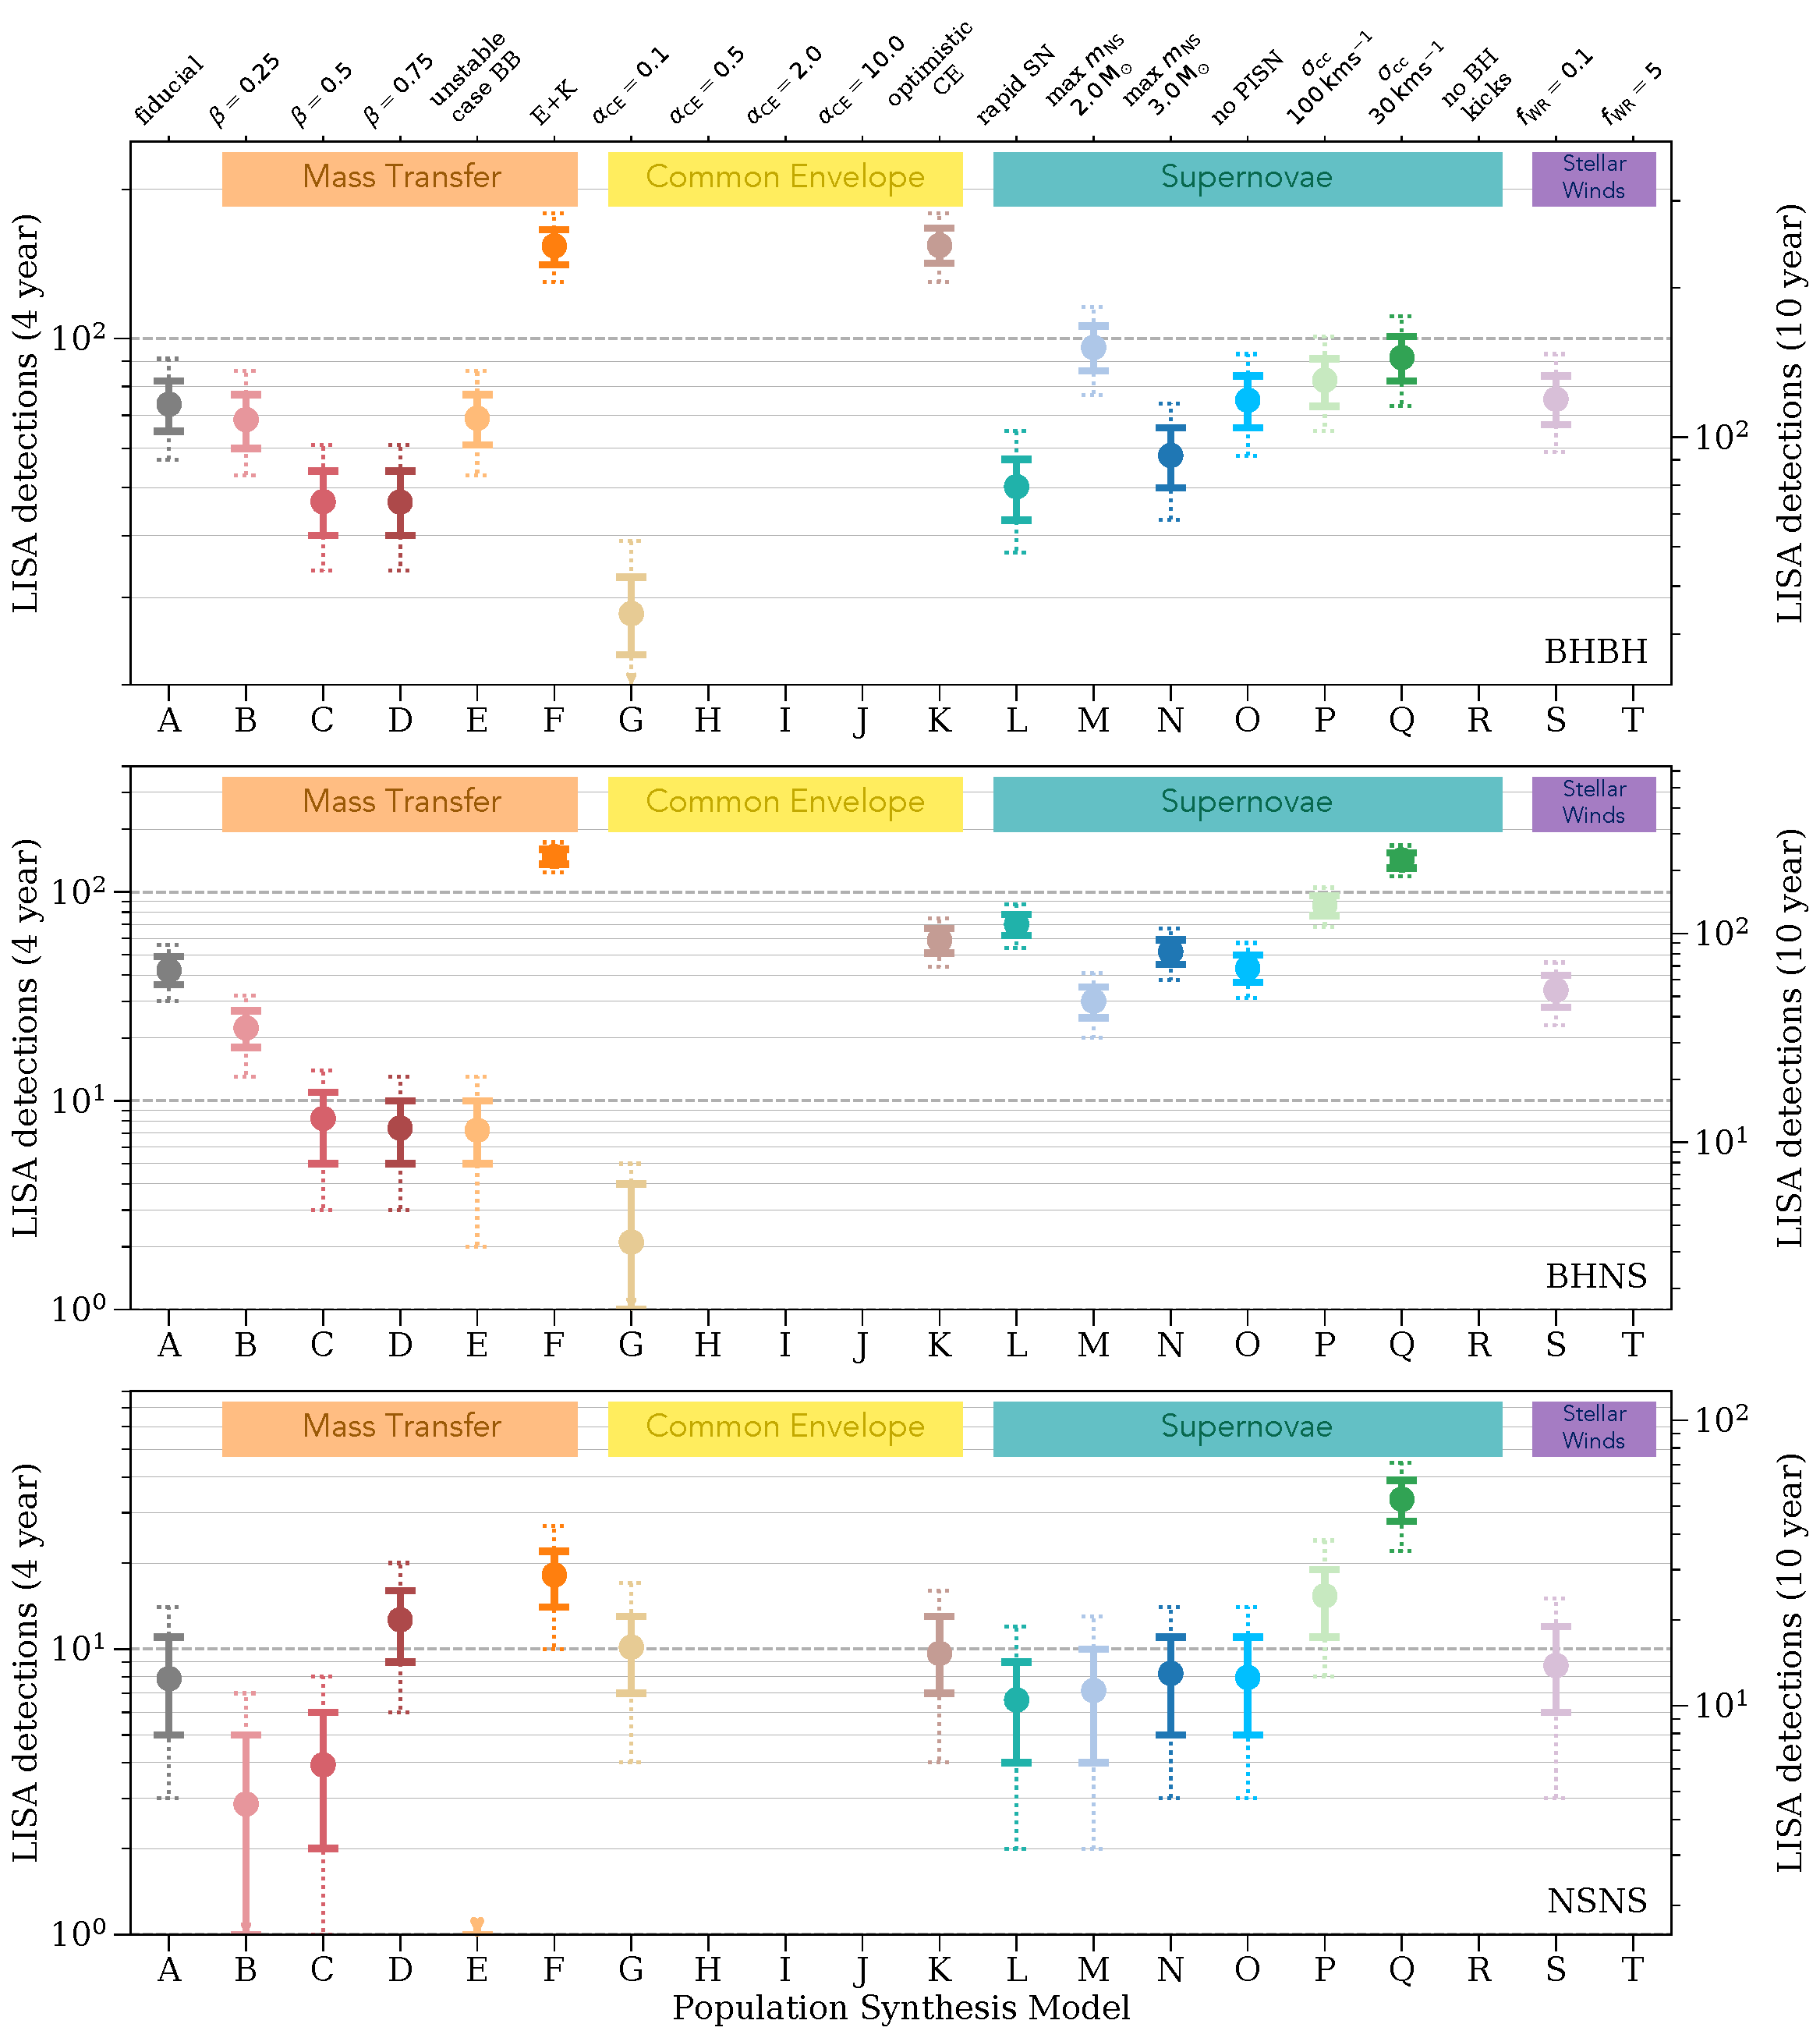
\includegraphics[width=\textwidth]{3_dco_detections.pdf}
    \caption{The number of expected detections in the LISA mission for different DCO types and model variations. Error bars show the 1- (solid) and 2-$\sigma$ (dotted) Poisson uncertainties. An arrow indicates that the error bar extends to zero. The left axis and grid lines show the number of detections in a 4-year LISA mission and the right axis shows an approximation of the number of detections in a 10-year mission (we scale the axis by $\sqrt{T_{\rm obs}}$, see Table~\ref{tab:detection_rates} for exact rates). Each model is described in further detail in Table~\ref{tab:physics_variations} and details of the fiducial assumptions are in Section~\ref{sec:fiducial_physics}. See Sec.~\ref{sec:detection_rate_analysis} for a discussion. \todo{Will add H, I, J, R, T once Floor says that they are done}}
    \label{fig:detection_rates}
\end{figure*}

\subsubsection{Mass transfer trends}

In models \modBetaLow{}-\modBetaHigh{}, we set the mass transfer efficiency $\beta$ to a fixed value. For the BHBHs and BHNSs, as we increase $\beta$ the detection rates steadily decrease. This may seem unintuitive since one may assume that a higher mass transfer efficiency would lead to more massive compact objects and thus a more detectable population. However, this contributes to the envelope mass and so without increasing the core mass or fallback rate, the final compact object mass is relatively unaffected. Moreover, one must consider that most of these DCOs are formed through a common envelope event and so retaining more of the envelope during mass transfer means that the eventual ejection of the envelope is much more difficult, thus leading to more stellar mergers and fewer detectable systems \citep[e.g.][]{Kruckow+2018}.

In contrast, for the NSNSs, the detection rate increases with increasing $\beta$. This is for two main reasons: firstly the ejection of a common envelope is less problematic for NSNSs as they are less massive \citep[e.g.][]{Kruckow+2018}. Moreover, the increased mass transfer efficiency means that systems that were previously below the mass necessary to become a NS can now accrete enough mass to form a NS. Although the same is true for more massive stars becoming BHs instead of NSs, due to the IMF, there is a net flux of more stars becoming NSs.

Enforcing that case BB mass transfer is always unstable (model \modCaseBB{}) has little effect on the BHBH detection rate whilst moderately and drastically decreasing the detection rates of BHNSs and NSNSs respectively. This is because a large fraction of NSs (and the majority of NSNS binaries are formed) through case BB mass transfer. Therefore, setting this mass transfer to be always unstable results in many of these binaries to merge before they could become DCOs since we assume the pessimistic CE scenario by default.

If we instead use the optimistic CE scenario when setting case BB mass transfer to be unstable (model \modCaseBBOpt{}) we find that the rates instead uniformly increase across DCO types. This is both from the natural increases from using the optimistic CE scenario (see Sec.~\ref{sec:detection_rate_CE_trends} in which we discuss model \modOpt{}), as well as additional increases from adding more DCOs formed through CE events after case BB mass transfer. This explains why we see more detections for BHNSs and NSNSs in model \modCaseBBOpt{} than in model \modOpt{}.

\subsubsection{Common envelope trends}\label{sec:detection_rate_CE_trends}

\subsubsection{Remnant mass prescription trends}

\subsubsection{Supernova kick trends}

\subsubsection{Stellar wind trends}

\subsubsection{BHBH detection rate trends}
The exception to this statement is model \modOpt{}, in which we allow Hertzsprung gap donors to survive common envelope events. A large fraction of the progenitors of BHs in this mass range expand significantly during the Hertzsprung gap phase and initiate common envelope events. Therefore, though the detectable fraction does not change significantly, the increased population of BHBHs in the Milky Way leads to this model predicting 2.5 times more detections.

\subsubsection{BHNS detection rate trends}

For the same reason as the BHBH rate, model \modOpt{} has a higher number of detections. This change is less prominent than in the BHBH case as the progenitors tend to be lower masses and initiate a CE event less frequently during the Hertzsprung gap phase. 

\tom{@ALL, the trend with common envelopes still confuses me, specifially, why does it not increase when $\alpha=2.0$? We never quite resolved this in the thread in zpro\_tom\_wagg with me and Lieke. I do see that the BHBH have a lot of only stable mass transfer and so reasonably are not too affected. NSNS basically only come through CE events and so sensibly are strongly affected but BHNS have $\sim 70\%$ classic channel and so should be affected strongly. But we don't see an increase with $\alpha = 2.0$. Any thoughts? (I'm leaving thinking about this for now in case it changes with the new data haha)}

The Fryer \textit{rapid} prescription (model \modRapid{}) leads to a higher detection rate for BHNSs because progenitors that would become black holes in the \textit{delayed} prescription, instead become neutron stars and so more BHNSs are formed instead of BHBHs. For the same reason, increasing the maximum neutron star mass (model \modNSHigh{}) increases the detection rate and the inverse is true when it is decreased (model \modNSLow{}).

Finally, models \modSigLow{}-\modNoBH{} show increased detection rates since lower kicks result in fewer disrupted binaries and hence a more numerous detectable population. Following this logic it makes sense that model \modSigLower{} produces more detections than model \modSigLow{}. The model with no BH kick (\modNoBH{}) is slightly lower than model \modSigLower{} as the number of surviving binaries is limited by the neutron star kick more than the black hole kick.

\subsubsection{NSNS detection rate trends}\label{sec:NSNS_detection_trends}

The vast majority of NSNSs in our sample are formed through the common envelope channel and thus changing the value of $\alpha_{\rm CE}$ has an effect on the rate. We see that decreasing $\alpha_{\rm CE}$ (model \modAlphaLow) leads to a lower rate as there is less energy available to eject the envelope and so more binaries result to stellar mergers rather than NSNSs and similarly we see an inverse trend when increasing $\alpha_{\rm CE}$ (model \modAlphaHigh).

As we found in the BHNS trends, a lower value for the core-collapse supernova velocity dispersion increases the detection rate in models \modSigLow{} and \modSigLower{}, whilst changing the PISN or BH kick prescription (models \modNoPISN{} and \modNoBH{}) of course has no effect on the NSNS population.

\subsection{Properties of detectable systems}\label{sec:property_variations}
\tom{This will be about how the shapes of the parameter distributions change for the different model variations. I won't detail every variation but I'll point out anything that stands out and leave the rest in the appendix plots.}
